
\chapter{Adjustment of Light Amounts}
\label{twoWaveplateTrick}

The light level from the master laser is constrained by our requirement that the Master laser operate single mode. However, we require control of the light levels further downstream in order to have the right light levels to avoid damage to the Acousto-Optic Modulator (AOM) and to have the right amount of light to injection lock the other lasers. 

A typical way to accomplish this is to install a half wave plate followed by a polarizing beam cube. In this way, one can take the linearly polarized incoming light and rotate its polarization to any angle. One can thus exert complete control of the amount of light coming out of the polarizing beam cube. 

We had initially intended to use this scheme. However, there was a mistake in placing the order. Instead of 0 order waveplates, we had received multi-order waveplates, whose performance rapidly degrades for wavelengths far from the specified wavelength. 

We could have easily ordered a 0 order waveplate to replace them. However, we found a way to use the exising waveplates.

\section{A review of the principles of operation of a waveplate: }

A waveplate rotates polarization by changing the relative phase of the oscillating components of the incoming polarized light. A waveplate has a fast axis and a slow axis. A half-wave plate is designed so that, at the specified wavelength, the component of polarization along the slow axis acquires a phase shift of $(2m+1)*\pi$ relative to the fast axis.Here $m$ is an integer. 

Recall that the phase acquired by light as it passes through a medium of index of refraction $n$ is given by 

\begin{equation}
  \Delta \phi = \frac{2 \pi n x}{\lambda} \label{deltaPhi0}
\end{equation}

Given indices of refraction of $n_1$ and $n_2$ for our two axes, we find that the difference in phase acquired by the components of the light's polarization will be 

\begin{equation}
\Delta \phi=\frac{2 \pi n_1 x}{\lambda} -\frac{2 \pi n_2 x}{\lambda}. \label{deltaPhi2}
\end{equation}

and we find that, in order to achieve the correct phase shift, the acceptable thicknesses of our half wave plate must satisfy

\begin{equation}
  \Delta \phi=(2m+1)\pi \label{deltaPhi1}
\end{equation}
where $m$ is the order of the waveplate.

Combining \ref{deltaPhi1} and \ref{deltaPhi2} we find that the thickness of a waveplate $x$ is given by

\begin{equation}
x=\frac{(2m+1) \lambda}{2 (n_1-n_2)}. \label{deltaPhi3}
\end{equation}


We now examine what will happen if we put a different wavelength than specified into the waveplate. Thus, we assume that $x$,$n_1$,$n_2$ and $m$ give the appropriate $\pi$ phase shift for the wavelength at which the waveplate is designed to work ($\lambda_s$). Now, we try light of a different wavelength, $\lambda'$. Assuming that the indices of refraction stay roughly the same for both $\lambda_s$ and $\lambda'$, we see that 

\begin{align}
\Delta \phi=\frac{2 \pi (n_1-n_2) x}{\lambda'} 
\end{align}
Then, taking $x\rightarrow ((2m+1) \lambda_s)/(2 (n_1-n_2))$ from Eq.\ \ref{deltaPhi3}, we get 
\begin{align}
\Delta \phi&=\frac{2 \pi (n_1-n_2) (2m+1) \lambda_s}{2 (n_1-n_2)\lambda'} \\
\Delta \phi&=\frac{\pi (2m+1) \lambda_s}{\lambda'} \label{deltaPhi4}
\end{align}
Eq.\ \ref{deltaPhi4} illustrates that the performance of a multi-order waveplate (with high value for $m$) will degrade more rapidly at different wavelengths than a low-order waveplate. 

\section{Motivation for use of two waveplates}
In our lab, we had a half wave plate, but it was a multi-order plate designed for 405 nm. Thorlabs specifies that the waveplates we had would provide the correct retardance at 405 nm, however they also specify that at 407.71 nm the net retardance is 0.3655746 waves, or $\Delta \phi=(m_2+.3656) (2 \pi)$. Based on Eq.\ \ref{deltaPhi4}, we see that this is consistent with and $m=55$ order waveplate. 

The problem here is that, in order to completely control the amount of light getting to the AOM, we want to change the polarization from fully vertical to fully horizontal. Given that the incoming light is vertically polarized, this retardance does not allow us to get fully horizontally polarized light, thereby imposing a minimum amount of light on us.

However, we found that we can compensate for this by simply using two waveplates in series. Using numerical methods, we found that the user can fix the orientation of one of the waveplates in such a way that by rotating the other waveplate over some reasonable distance (i.e. over a range of angles large enough that a user could adjust the waveplate by hand), the outgoing light can be smoothly adjusted between being completely vertical or completely horizontal. 

Now, the polarization of the light when it is neither completely vertically nor completely horizontally polarized will not necessarily be linearly polarized. There will, in general, be some arbitrary phase shift between the components of polarization. However, this does not matter for our purpose since the goal was simply to control the amount of power exiting from each of two sides of a polarizing beam cube. 

\section{Jones Matrices}
This can be demonstrated using the Jones matrix formalism. The polarization of the incoming light can be represented by the following Jones vector: 
\begin{equation}
\begin{pmatrix}
0\\1
\end{pmatrix}
\end{equation}

The Jones matrix corresponding to our waveplate is easily derived. Given that: 

\begin{multline}
\begin{pmatrix}
\cos\theta & - \sin \theta \\
\sin \theta & \cos\theta \\
\end{pmatrix}
\begin{pmatrix}
\xi & 0 \\
0 & 1 \\
\end{pmatrix}
\begin{pmatrix}
\cos\theta &  \sin \theta \\
-\sin \theta & \cos\theta \\
\end{pmatrix} \\
=
\begin{pmatrix}
\cos ^2 \theta+\xi \sin^2 \theta &  \cos\theta \sin \theta-\xi \cos\theta \sin \theta \\
\cos\theta \sin \theta-\xi \cos \theta \sin\theta & \xi \cos^2 \theta + \sin^2 \theta \\ \label{JonesMatrix001}
\end{pmatrix}
\end{multline}

where $\theta$ is the angle between the fast axis and the x axis. 

We let $\xi\approx e^{.366 (2 \pi)}$ as specified by the waveplate. Then, to represent two of them mounted at angles $\theta_1$ and $\theta_2$ respectively, we need merely multiply two matrices like the one in Eq.\ \ref{JonesMatrix001}. Writing out the result is straightforward, but we left it to a computer algebra system.

By numerical experimentation, we found that there was a set of angles where we could mount our two waveplates that would result in a polarization for the outgoing light that is orthogonal to the polarization of the incoming light. 

\begin{figure}
    \centerline{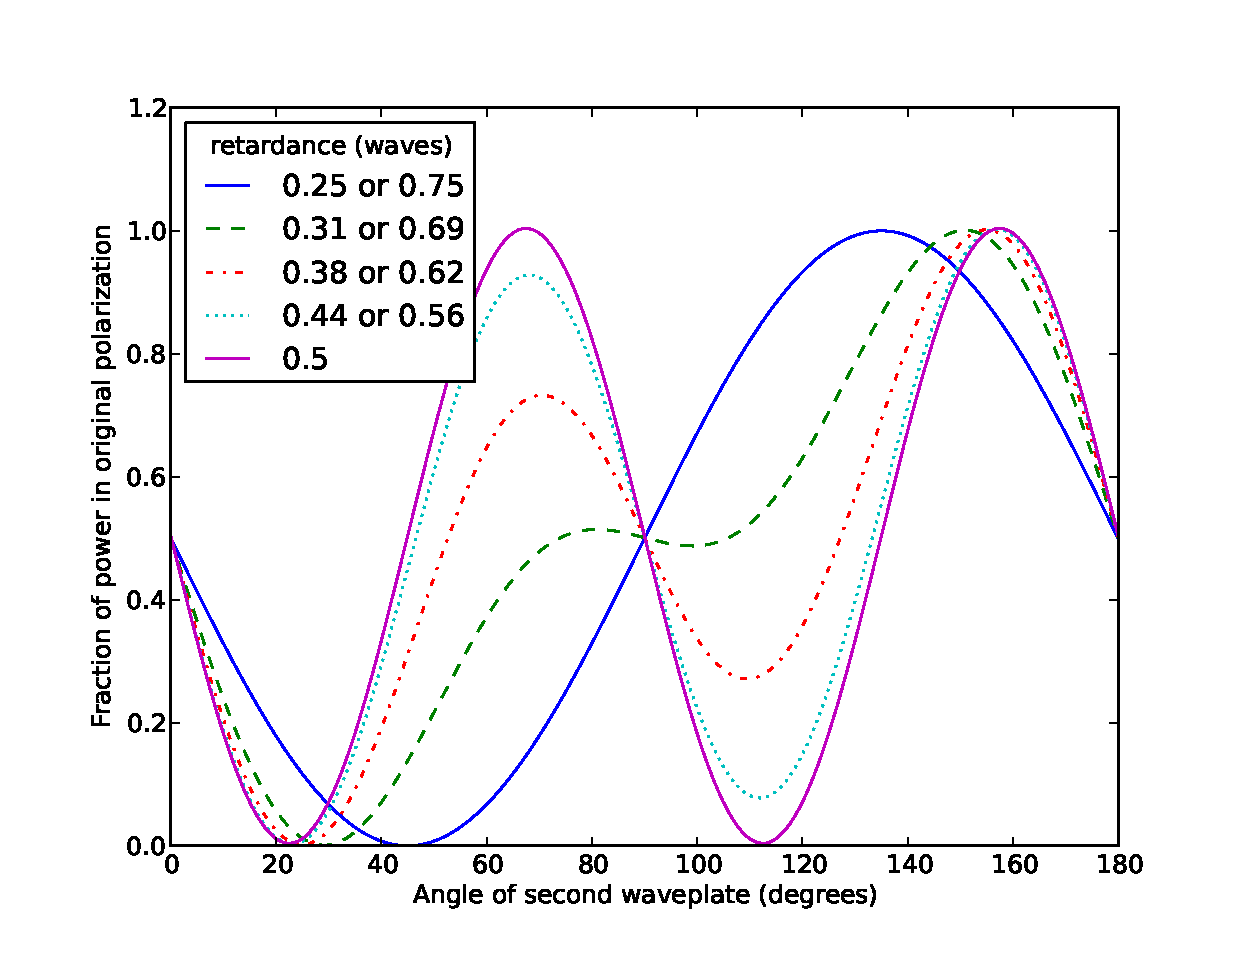
\includegraphics{NewNotesSymmetricFig}}
    \caption[Numerical method]{\label{fig:numericalLightControlMethod}
    A plot the magnitude of the fraction of the power at the original polarization as a function of the angle of the second waveplate for various retardances.}
\end{figure}


\section{Alignment Procedure}
By physical and numerical experimentation, we found that you can achieve these angles by subsequently adjusting each of the two waveplates in turn. Keeping 100\% of the light vertically polarized is easy and can be achieved for any fixed value of $\theta_2$ since $\theta_1$ can simply be adjusted so that the fast axis of the first waveplate aligns with the slow axis of the second. In this way, the total phase shift experienced by all the components is equal.

Thus, to correctly place the second waveplate at the angle  $\theta_2$, we adjust both angles until the outgoing light is entirely horizontally polarized (as measured by the output of the polarizing beam cube). I found that mounting the waveplates at the approximate angles I calculated followed by alternately adjusting each waveplate to minimize the amount of light transmitted achieved the desired result. 

\section{Results for other combinations of waveplates}
We performed additional numerical calculations and found a couple things:

This only works for certain retardances. If one of the waveplates has a retardance of 0.5 waves, then (obviously) this would work. If the two waveplates have the same retardance and that retardance is between 0.25 and 0.75 waves, this will also allow the user to put anywhere from 0\% to 100\% of the power into either polarization. Figure\,\ref{asymmetric} illustrates the maximum power that can be extinguished as a function of the retardance of the two waveplates.


\begin{figure}
    \centerline{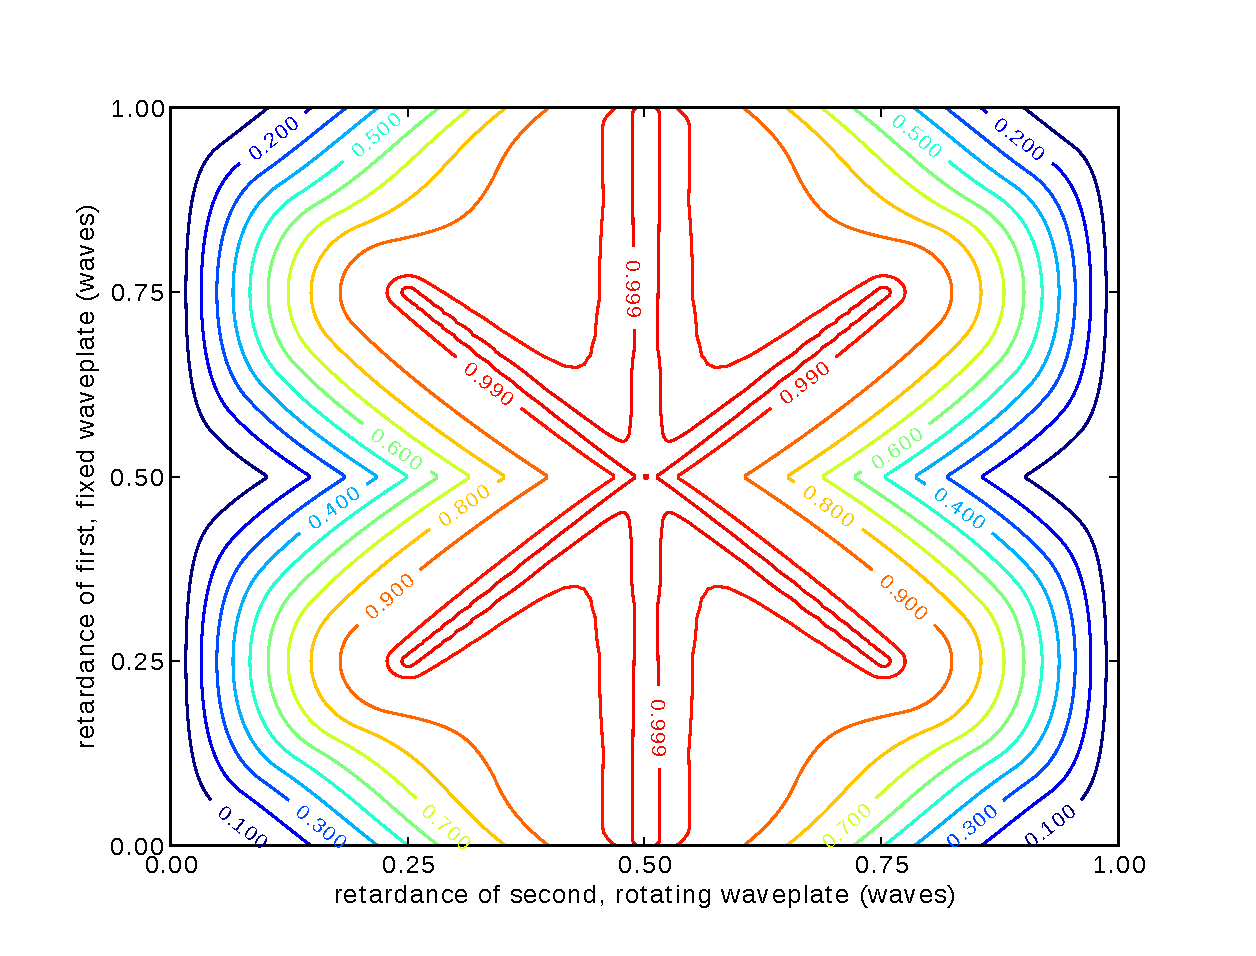
\includegraphics{NewNotesAsymmetricFigure}}
    \caption[Numerical method]{\label{asymmetric}
   The maximum power that one can extinguish through the polarizing beam cube given the retardance of the two waveplates. As one expects, if either waveplate has a retardance of 0.5 waves, one can get the full range of possible outgoing polarizations. However, this is only possible for certain combinations of waveplate retardances}
\end{figure}

\section{Attempt at building intuition}

Armed with the important clue that the we can use this trick only if the waveplates have the same retardance, we can make an attempt at describing the phenomenon only in terms of symmetry arguments.

We first consider vertically polarized light travelling into a waveplate. If we align the fast axis of the waveplate to the vertical direction, our vertically polarized light will emerge with a vertical polarization. 

However, if we rotate the fast axis to one side by some angle $\theta$, we get elliptically polarized light. Notice tht if we rotate the fast axis to the other side (i.e. by some angle $-\theta$) we also get elliptically polarized light. However, this light is elliptically polarized with the same ellipticity, but with the opposite handedness.

Now, we consider the second waveplate. We would like to consider what it would take to get horizontally polarized light coming out of the second waveplate. We can do this by noting that our system has time reversal symmetry. The time reversed outgoing horizontally polarized light turns out to be incoming horizontally polarized light. Similarly as before, the second waveplate can achieve elliptically polarized light of various handednesses.

Now, we simply argue that, by symmetry, we can place the two waveplates at some set of angles such that the elliptically polarized light coming out of the first waveplate corresponds to the time reversed elliptically polarized light coming through the second waveplate. It turns out that this leads to a nice symmetry in the result where, in order to get linearly polarized light out of the whole apparatus, the angle between the incoming polarization and the fast axis of the first waveplate will be equal in magnitude but opposite in sign to the angle between the outgoing polarization and the fast axis of the second waveplate.
%maybe do it differentially? You know? 

%let it be imperfect. Use other time for cleverness. Take advantage of having idea net out. 
%should I find a commutator? 
%IDK if I did this right with my \xi
%don't forget to cite peatrossware
%http://www.thorlabs.com/NewGroupPage9.cfm?ObjectGroup_ID=713 is where I got the spreadsheet. 
